\section{Background}

In the following experiment we will use a diode laser to measure the absorption
spectrum of rubidium. Due to their small size, high efficiency and tunability,
diode lasers are of a great scientific interest.
In the following chapters, the basic principle
of a general laser system will be considered before discussing the specific
properties of a diode laser.

\subsection{General lasing system}

In this chapter we will look at the main interaction between light and a
quantum mechanical system like an atom. In atoms the electrons possess different
dicrete energy levels. Nontheless, to discuss the main principle of a laser
we will use a system with only two energy levels shown in figure \ref{fig:twolevelsystem}.
By absorbing a photon, an electron can be excited from the lower state to the
higher state (figure~\ref{fig:twolevelsystem} a).
The relaxation back into the ground state can be radiative or
nonradiative.
\begin{figure}
  \centering
  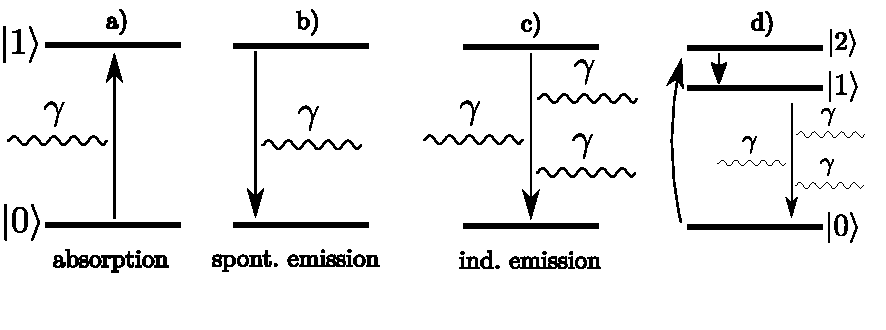
\includegraphics[width = \textwidth]{Pics/energyscheme.pdf}
  \caption{Figures a) - c) show the fundamental interactions of light with a
  quantum mechanical system: absorption, spontaneous emission and induced emission.
  Figure d) shows the three level system required for the population inversion
  \cite{steven}.}%https://github.com/stefangri/s_s_masterpraktikum/blob/master/V60_Diodenlaser/report/pics/energyscheme.pdf
  \label{fig:twolevelsystem}
\end{figure}
In nonradiative relaxation processes the remaining energy will be converted into
heat by phonon scattering. In a radiative relaxation process the energy will
be displaced by emitting a photon. This can happen spontaneous (Figure \ref{fig:twolevelsystem} b)
or stimulated by an incoming photon (Figure \ref{fig:twolevelsystem} c).
Therefore the energy of the incoming photon must be the difference between the
two states. As a result there will be two photons emitted with the same phase,
direction and energy. This process called 'stimulated emission' is necessary
for constructing a lasing system. To reach a higher propability for 'stimulated emission'
than 'spontaneous emission' the population of the second state has to be higher
than the ground state. This situation is called 'population inversion'.

Although the principle of a lasing sytem was explained by using a two state system,
for constructing a real laser at least three energy levels are necessary. The population
of a single energy level is given by the boltzmann-distribution:
\begin{equation}
    \frac{N\ua{2}}{N\ua{1}} = e^{\frac{E_1-E_2}{k\ua{B}T}}\quad \underset{T \rightarrow \infty}{\longrightarrow}\quad  1, \quad E\ua{2}>E\ua{1}.
    \label{eqn:pop}
\end{equation}
The only
parameter which can be changed is the temperature. It´s easy to see, that even
by heating up the system to an infinite temperature, only an equal population
of both states in a two level system is possible (\ref{eqn:pop}). In the three level system
shown in figure~\ref{fig:twolevelsystem} d),
electrons will be excited into the highest state by using a external pump source.
The lifetime of the second state has to be much lower than the lifetime of the
first state to create a population inversion. The relaxation from the first state
into the ground state is called 'lasing transition'.

\subsection{General laser system}

A lasing system basically consists of four main components. The first one is the
active lasermedium. It determines the wavenlegths which can be generated by the
system. In this experiment we use a semiconductor, but it is also possible to
uses gases like Helium. The properties of semiconductors as a laser medium will
be discussed later on.

The second main component is the cavity. The cavity is formed by two reflective
surfaces of which only one is fully reflective. The other one is only partially
reflective and is used as the output coupler. In cause of the reflective surfaces
athe light passes the medium multiple times and a  standing wave will be formed.
Only dicrete longitudinal modes are allowed inside the cavity which are defined
by the cavity length and the wavelength:
\begin{equation}
  L = \frac{\lambda}{2}\cdot n \;\;, \;\; n \in \mathbb{N}.
  \label{eqn:cavitylength}
\end{equation}
The difference between two antinodes can be easily derived from the equation
above and can also be expressed by using the frequency of the laser $\nu$:
\begin{equation}
  \increment \lambda = \frac{v}{\increment \nu} = 2L \Leftrightarrow \increment \nu = \frac{v}{2L} = \frac{c}{2nL}.
  \label{eqn:frequdiff}
\end{equation}
The parameter $v = \sfrac{c}{n}$ is the speed of light in the cavity medium,
which is the speed of light $c$ divided by the refrective index $n$ of the used medium.
By manipulating the cavity length it is possible to change the wavelength with the
most gain. The wavelength distribution of the laser medium is typically much broader
than the difference between two longitudinal modes. To intensify only one specific mode
and generate a laser with a sharp wavelength broadwith, it is usual to combine
different cavities. The distribution of each cavity will be multiplied, so that
only at a specific wavelength the gain is higher than the losses.

The third main component is the pump source for creating the
population inversion. In diode laser systems the pump source is given by a
current. The specific functionality will be discussed in the next chapter.
The fourth and last necessary component is the cooling system, which
description is not a topic of this transcript.

\subsection{Functionality of a diode laser}

In the following chapter we will first take a look at the properties of
a semiconductor as an active laser medium. Than we will discuss the specific
laser setup, which is used at this experiment.
\begin{figure}
  \centering
  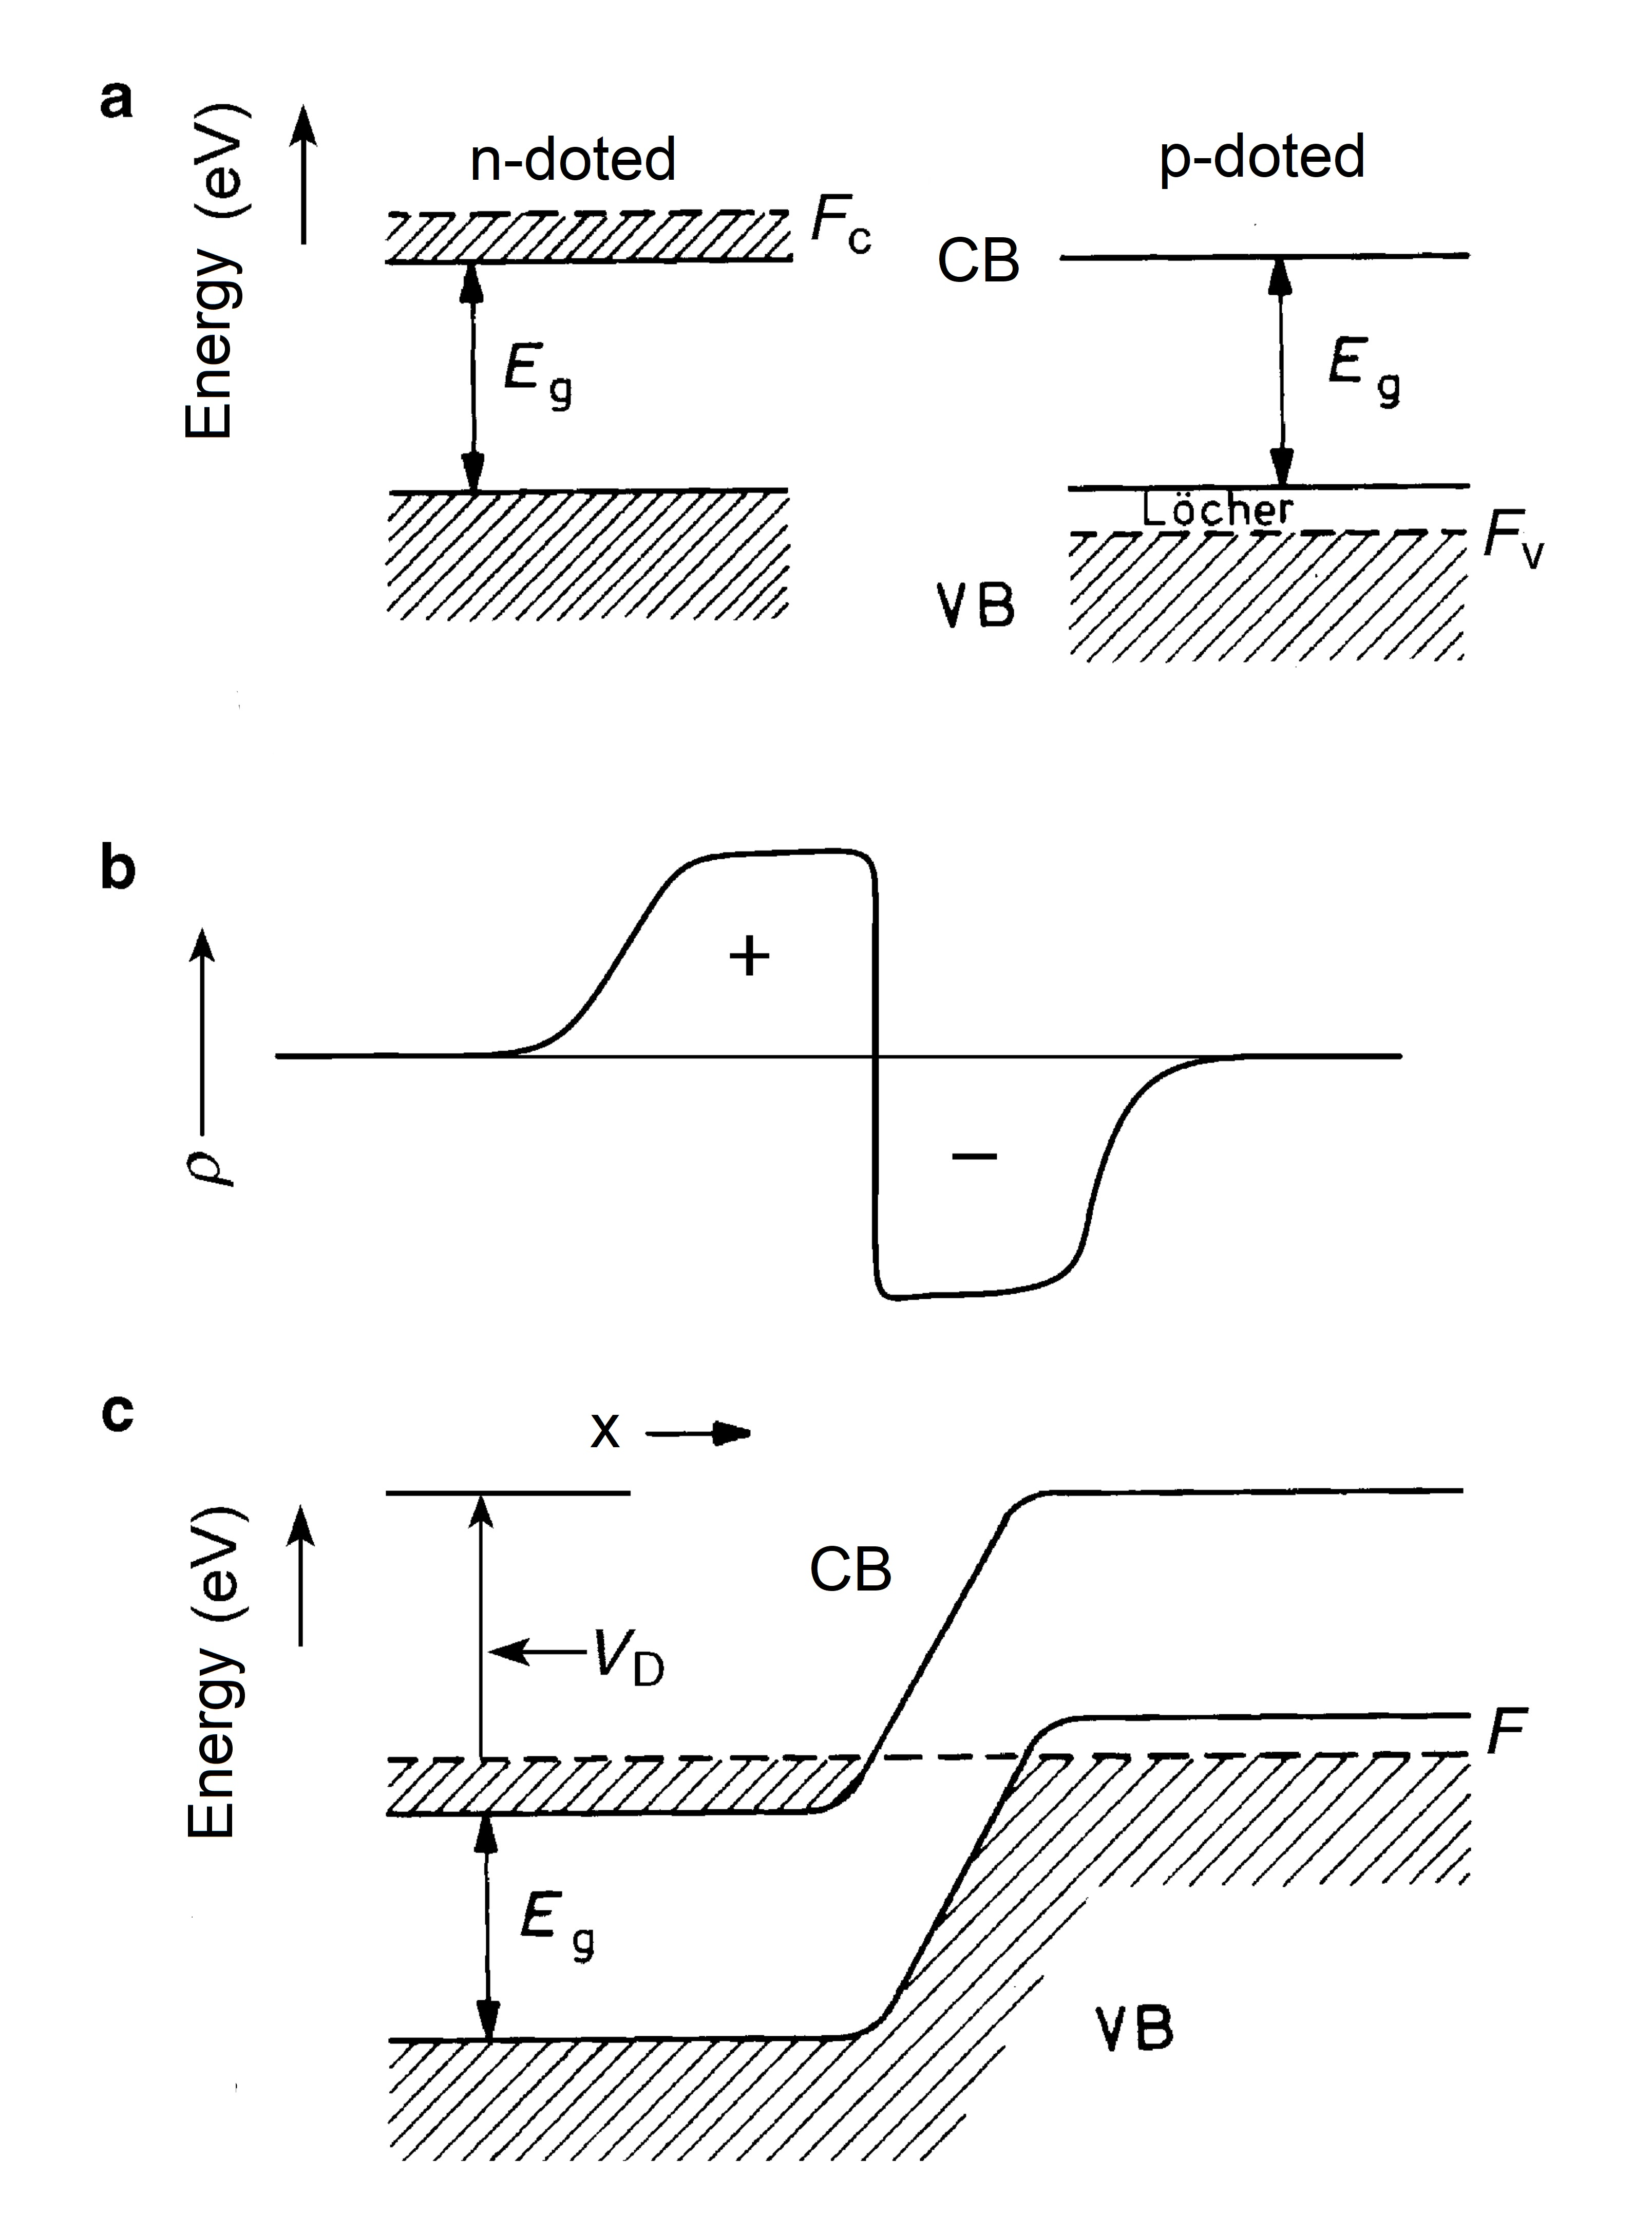
\includegraphics[width=0.5\textwidth]{Pics/doted.jpg}
  \caption{a) band scheme for n- and p-doted areas in a semiconductor. b)~space
  charge density and c)~schematic band structure for connected n- and
  p-doted areas \cite{Eichler}.}
  \label{fig:n_p_doted}
\end{figure}
A semiconductor is a solid material with a band gap below four electron volts
$E\ut{gap}~<~\SI{4}{\electronvolt}$ between the highest valence band and the
lowest conduction band. By doping a semiconductor with different atoms it is
possible to increase the density of positive or negative charge carriers. The
resulting band scheme for both types is shown in figure~\ref{fig:n_p_doted}.
Due to the current induced by the applied voltage the potential difference
between the two different doted materials will be reduced so that the radiative
recombination of electrons and holes is possible (figure~\ref{fig:appliedcurrent}).
Therefore the used material must be a direct semiconductor. By increasing the
applied voltage its possible to create a higher intensity of the emitted photons.

It is important to mention that the laser active only starts above a
specific current threshold $I\ut{th}$ and lhe laser power is limited due to joule
heating (figure~\ref{fig:current}). Below the threshold the losses exceed the gain
and the light-ouput is based mainly on spontaneouse emmission. A population
inversion can not be achieved in this case. Also the Bandgap of a semiconductor
depends on the temperature, which is the reason that varying the temperature
also changes the wavelength of the emitted photons.
\begin{figure}
  \centering
  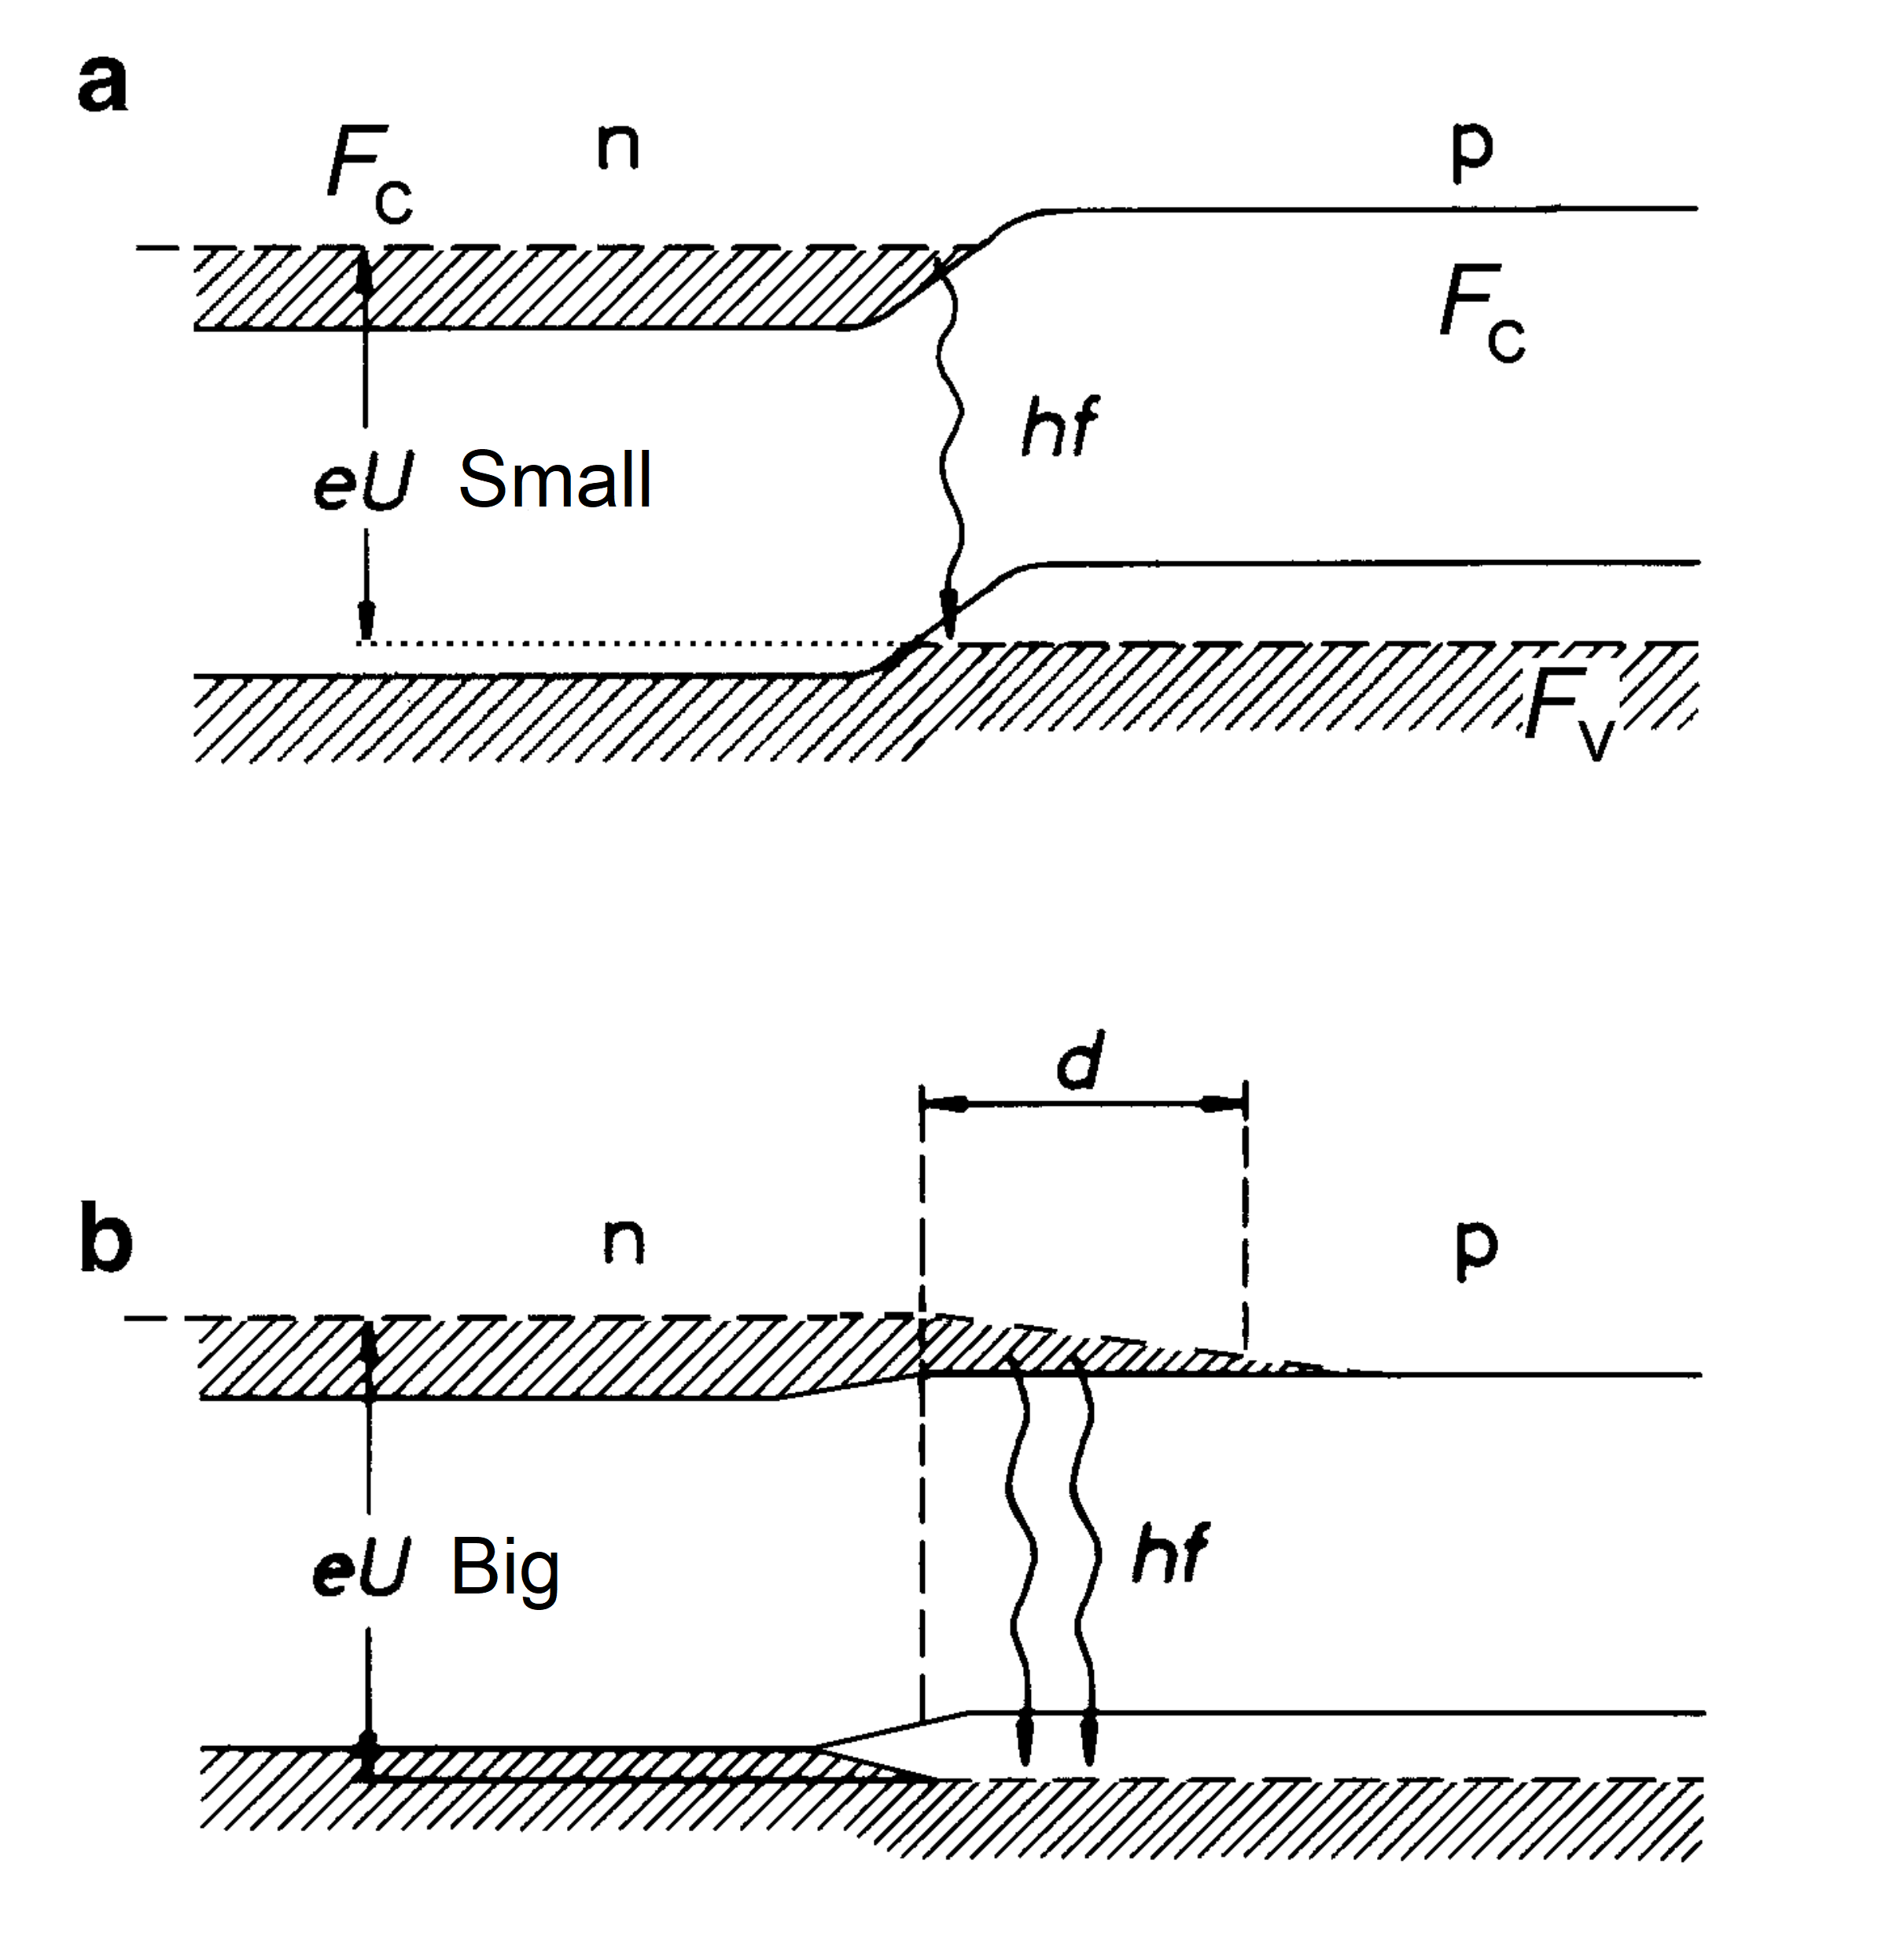
\includegraphics[width = 0.6\textwidth]{Pics/appliedcurrent.png}
  \caption{Radiative emission in cause of recombination at different voltage levels.
  \cite{Eichler}.}
  \label{fig:appliedcurrent}
\end{figure}
\begin{figure}
  \centering
  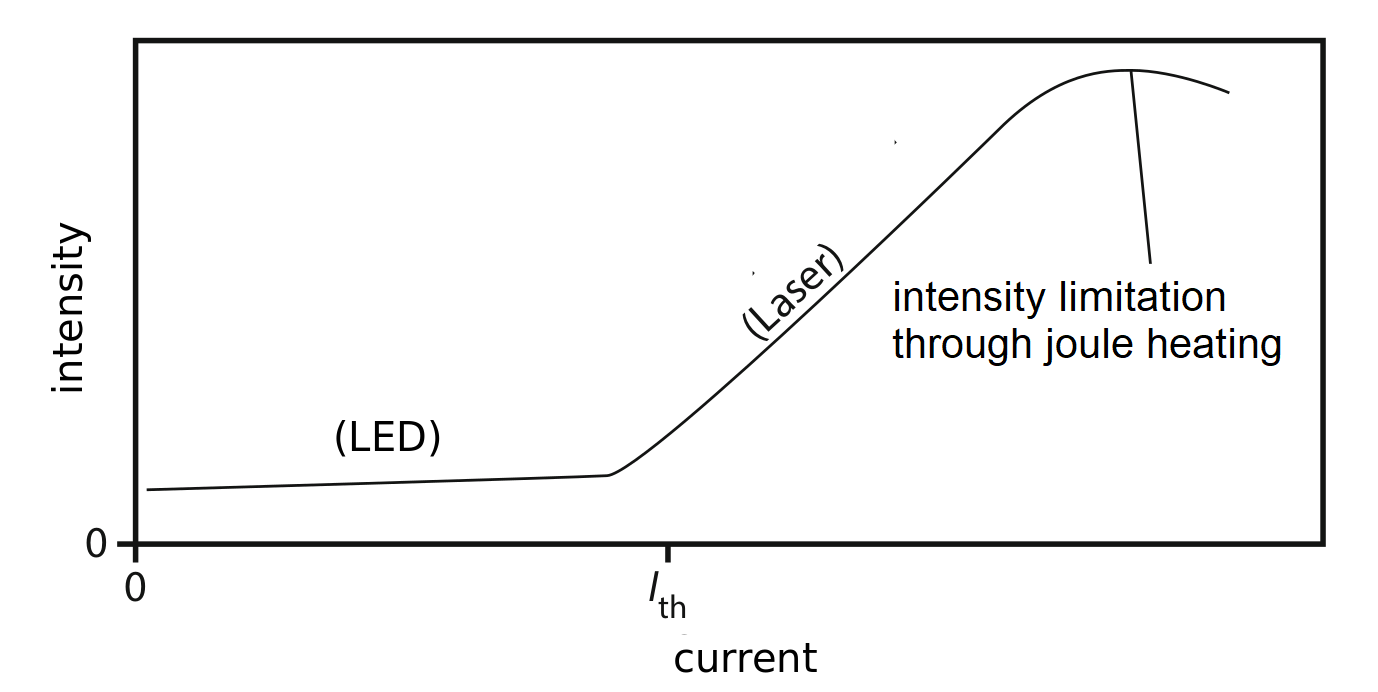
\includegraphics[width = 0.7\textwidth]{Pics/current.png}
  \caption{Relation between output intensity and the applied current. The laser
  activity starts above the thereshold and is limited due to joule heating.\cite{Eichler}.}
  \label{fig:current}
\end{figure}

To reduce the losses inside the diode chip in cause of emitted photons entering
non active layers, often different structres to guide the light are used.
One possibility is the gain-guided structure, where the current passes only a
small part of the active layer. The other possibility can be acheived by limiting
the active layer itself spatial (index-guided-structure). Both Structures are
shown in figure~\ref{fig:guided}.
\begin{figure}
  \centering
  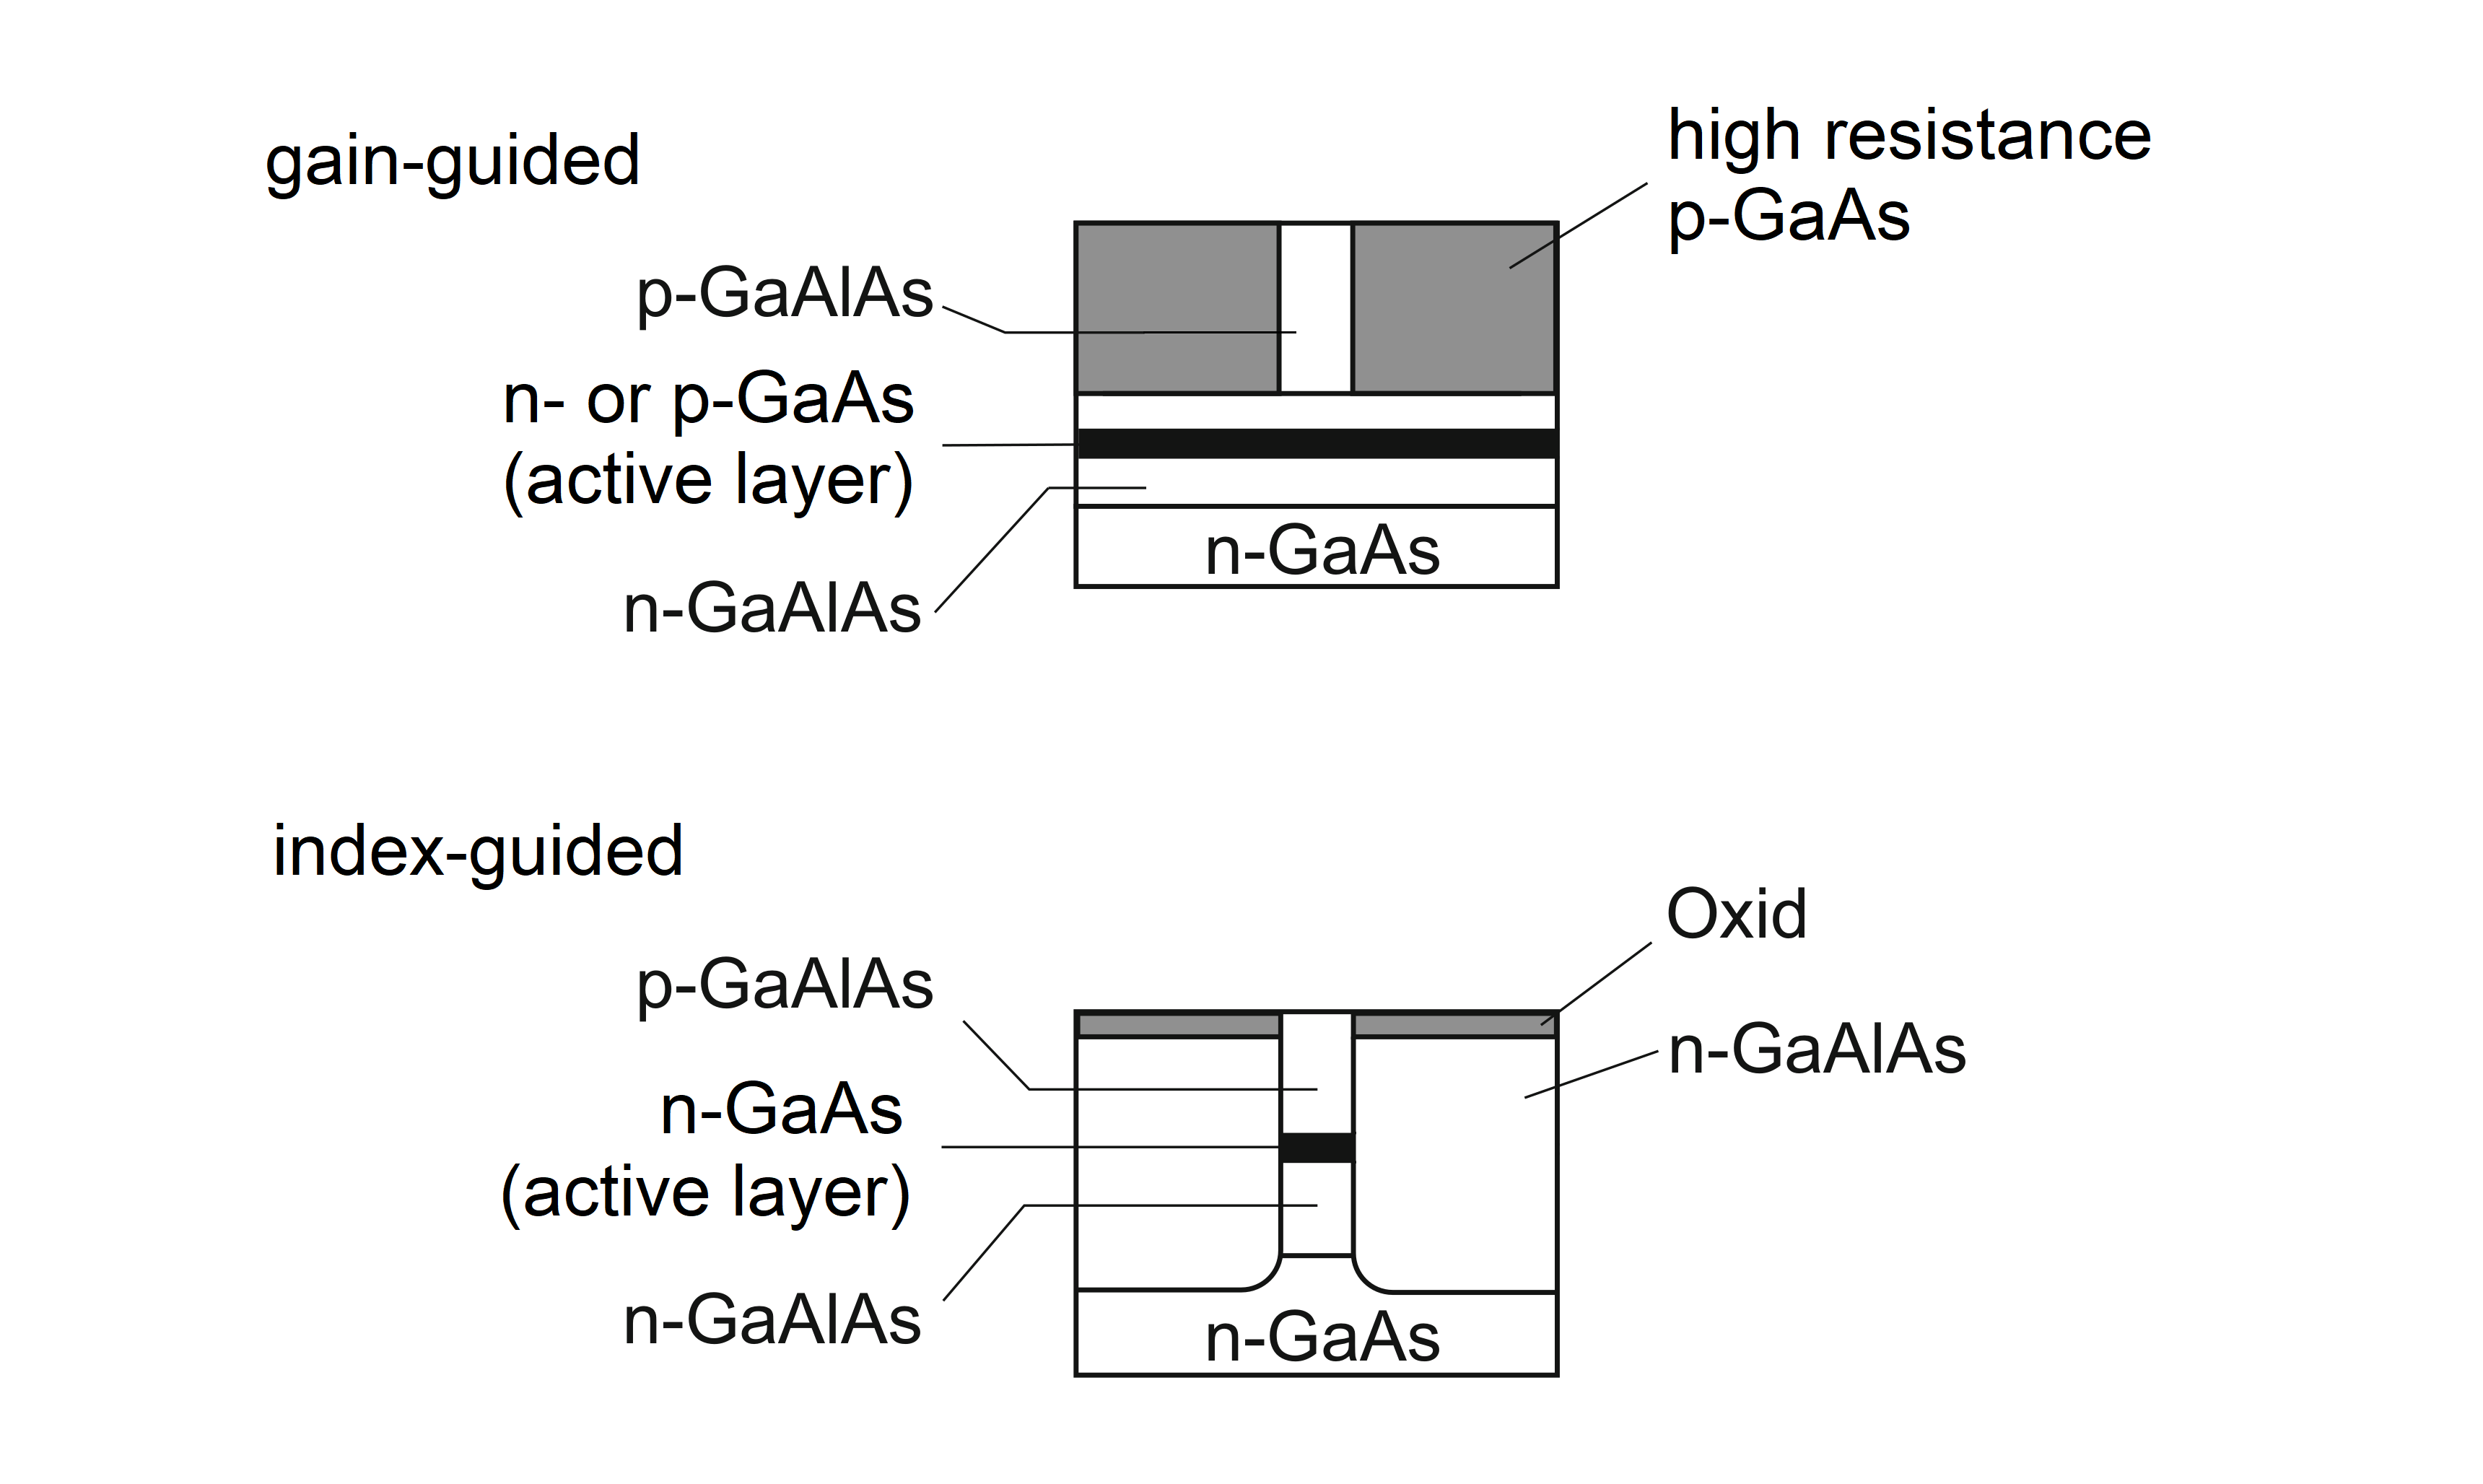
\includegraphics[width = \textwidth]{Pics/guided.png}
  \caption{Two different heterostructures where guiding of the emitted light is
  enabled. Figure a) shows a possible realisation of a gain-guided by blocking
  the current from the active layer. Figure b) shows a index-guided structre in
  which the active layer is limited spatially \cite{Eichler}. }
  \label{fig:guided}
\end{figure}
\begin{figure}
  \centering
  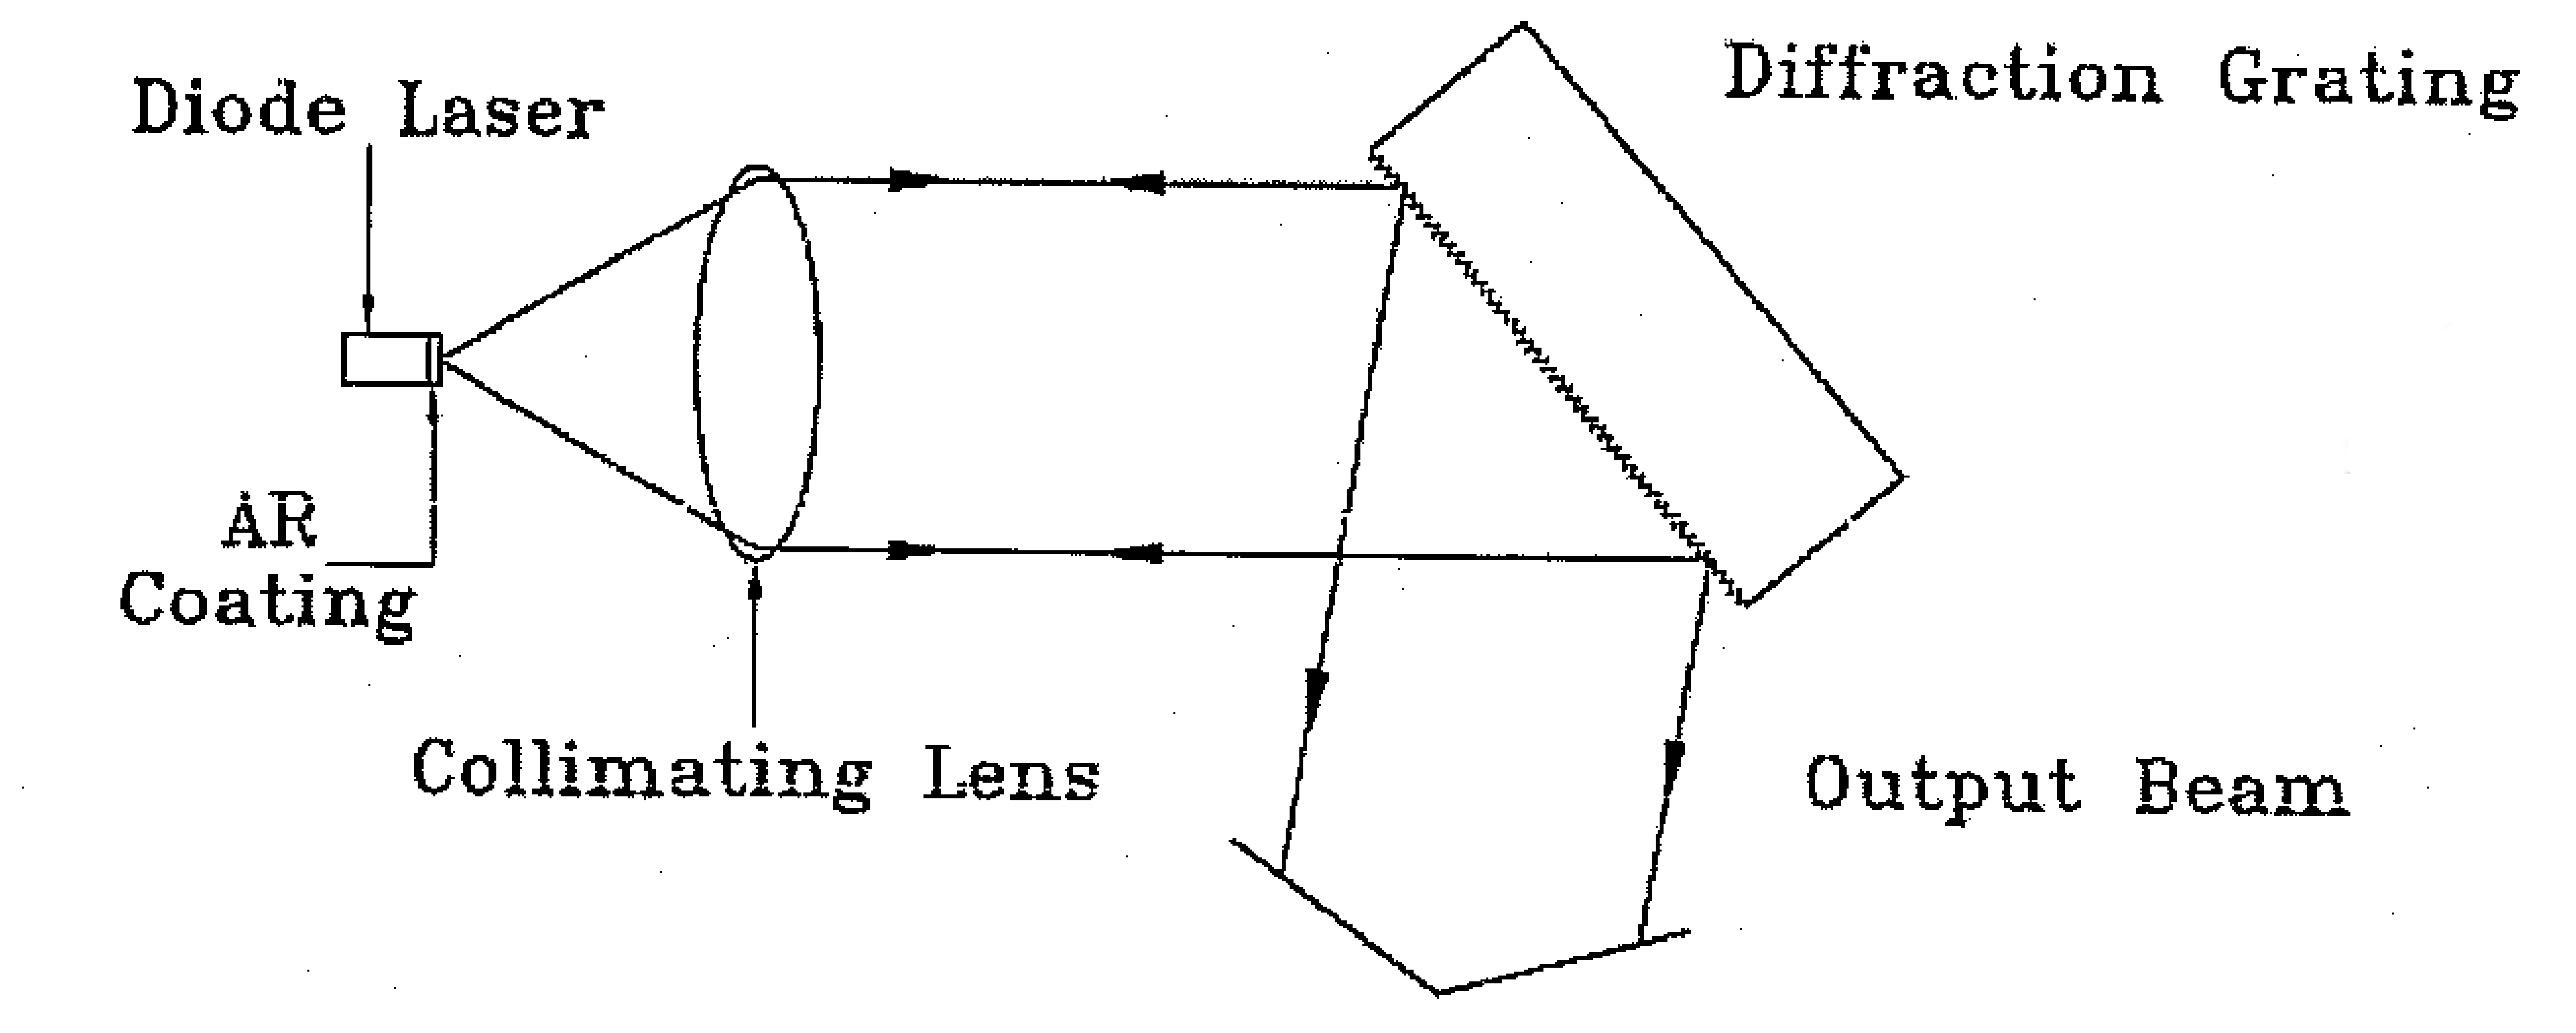
\includegraphics[width = 0.9\textwidth]{Pics/setup.png}
  \caption{Basic configuration of the used diode laser system \cite{anleitung}.}
  \label{fig:setup}
\end{figure}

The setup described in the following paragraph is shown in figure \ref{fig:setup}.
The emitted photons from the active layer are strongly divergent. For this reason
a collimating lens is placed behind the diode laser chip. The setup consists of
two different cavity. The first one is the cavity formed by the two reflective ends
of the diode chip. The coupling output is in the direction of the collimating lense.
The second cavity is formed by the rear end of the chip and the grating. The length
between chip and grating is variable so that the wavelength can be varyied. Additionally
by reflect different deffraction maxima into the active layer. The resulting
gain distribution can be seen in figure \ref{fig:gain}
\begin{figure}
  \centering
  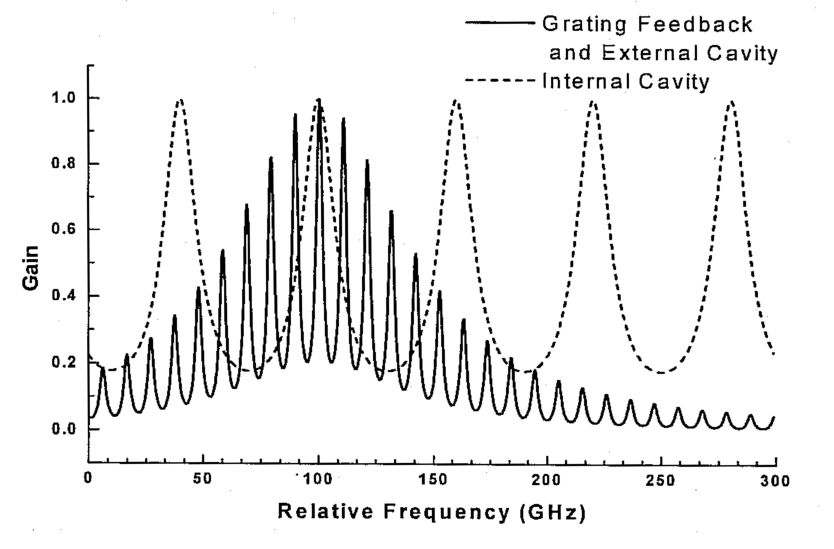
\includegraphics[width = 0.7\textwidth]{Pics/gain.pdf}
  \caption{Gain distribution for the different components used in this setup \cite{anleitung}.}
  \label{fig:gain}
\end{figure}
